\documentclass{article}
\title{Math 466 - Numerical Methods: Project 2}
\author{Thomas Simcox}
\date{Fall, 2021}

\usepackage{amsmath, amsfonts, amssymb, amsthm, fancyvrb, graphicx}
\usepackage[margin=1.5in]{geometry}


\begin{document}
    \vspace{30em}
    \maketitle
    \begin{center}
        \fbox{ My full \texttt{.jl} file can be found on my Github at the following link:  }
    \end{center}


    \vspace{3em}

    \section*{1a}
    Let $A \in \mathbb{R}^{n\times n}$ and consider the iteration
    \begin{align*}
        X_{k+1} = \frac{1}{2}\left(X_k + \left(X_k^{-1}\right)^{\top}\right) \,\,\text{  where  }\,\, X_0 = A.
    \end{align*}
    Write a program to perform this iteration and test your program with the input
    \begin{align*}
        A\,\,=\,\, \begin{bmatrix}
            -0.49 & -0.21 & -0.40 & -0.21\\[.5em]
            0.36 & 0.10 & 0.29 & -0.04\\[.5em]
            0.12 & -0.01 & 0.48 & -0.47\\[.5em]
            0.09 & 0.09 & -0.41 & 0.22\\
        \end{bmatrix}
    \end{align*}
    Verify the Frobenius matrix norm $||X_0 - X_1||_F \approx 16.37054203598731$.\\
    
    \newpage
    \begin{Verbatim}[frame=single, label=Find first iteration, numbers=left, fontsize=\small, xleftmargin=-.5cm, xrightmargin=-0.5cm, framesep=3mm]
      #######################################
      # 1a.

      # function that calculates next iteration
      pol! = (A::Matrix{Float64}) -> (A + (inv(A))') / 2;
      
      # driver function that finds the n'th iteration
      function pol_driver(A::Matrix{Float64}, n::Int64)::Matrix{Float64}
          B = copy(A)
          for i = 0:n
              B = pol!(B)
          end 
          return B;
      end 
    \end{Verbatim}
    \vspace{2em}
    \begin{Verbatim}[frame=single, label=Julia REPL for first iteration, numbers=left, fontsize=\small, xleftmargin=-.5cm, xrightmargin=-0.5cm, framesep=3mm]
    julia> include("polar.jl")
    ||X_0 - X_1|| = 16.37054203598732
    \end{Verbatim}

    \newpage

    \section*{1b}
    Define $\Delta_k = X_{k+1} - X_k$. If $X_k$ converges then it follows that $\Delta_k \to 0$ as $k \to \infty$. Compute $||\Delta_k||_F$ for $k = 0, \ldots, 9$.
    \vspace{3em}
    \begin{Verbatim}[frame=single, label=Find and print Delta k, numbers=left, fontsize=\small, xleftmargin=-.5cm, xrightmargin=-.5cm, framesep=3mm]
        #######################################
        # 1b.

        # compute delta_k 
        delta_k = (X, k) -> pol_driver(X, k) - X;
                                 
        # store all the delta_k's in a list for k = 0:9
        delta_ks = [delta_k(copy(A), k) for k = 0:9];
       
        # display the norm of each delta_k
        map(x -> "||Delta_k|| = $(norm(x))", delta_ks);

    \end{Verbatim}

    \vspace{1em}

    \begin{Verbatim}[frame=single, label=Julia REPL for Delta k, numbers=left, fontsize=\small, xleftmargin=-.5cm, xrightmargin=-.5cm, framesep=3mm]
        10-element Vector{String}:
         "||Delta_k|| = 16.37054203598732"
         "||Delta_k|| = 8.218875822891379"
         "||Delta_k|| = 4.207915072995769"
         "||Delta_k|| = 2.325403875547138"
         "||Delta_k|| = 1.5563638515455411"
         "||Delta_k|| = 1.3312012593101599"
         "||Delta_k|| = 1.3023069956996867"
         "||Delta_k|| = 1.301756540894667"
         "||Delta_k|| = 1.3017563374673147"
         "||Delta_k|| = 1.3017563374672871"
    \end{Verbatim}

    \newpage

    \section*{1c}
    Suppose $X_k$ is $\alpha$-order convergent such that $||\Delta_{k+1}||_F \approx M||\Delta_k||_F^\alpha$. Then
    \begin{align*}
        \log ||\Delta_{k+1}||_F \,\, \approx \,\, \log M + \alpha \log ||\Delta_k||_F
    \end{align*}
    would show $\log ||\Delta_{k+1}||_F$ is a linear function of $\log||\Delta_k||_F$. Plot the points
    \begin{align*}
        \left(\log ||\Delta_k||_F \,,\, \log ||\Delta_{k+1}||_F\right) \,\,\text{  for  }\,\, k = 1, \ldots, 8.
    \end{align*}
    Do all the points fall on a line? Find the slope between the last two points by computing
    \begin{align*}
        \alpha \approx \frac{\log||\Delta_9||_F - \log ||\Delta_8||_F}{\log||\Delta_8||_F - \log ||\Delta_7||_F}
    \end{align*}
    \vspace{1em}
    \begin{Verbatim}[frame=single, label=Plot Delta k Points, numbers=left, fontsize=\small, xleftmargin=-.75cm, xrightmargin=-.75cm, framesep=3mm]
    #######################################
    # 1c.
  
    # plot log of delta_ks
    plot(log_delta_k, markershape = :circle, markercolors = :white, label="||Delta_k||")
  
    # find slope of last two points
    alpha = log_delta_k[9] - log_delta_k[8] / log_delta_k[8] - log_delta_k[7]

    # print alpha
    println("Slope between last two points: Alpha = $alpha")
    \end{Verbatim}
    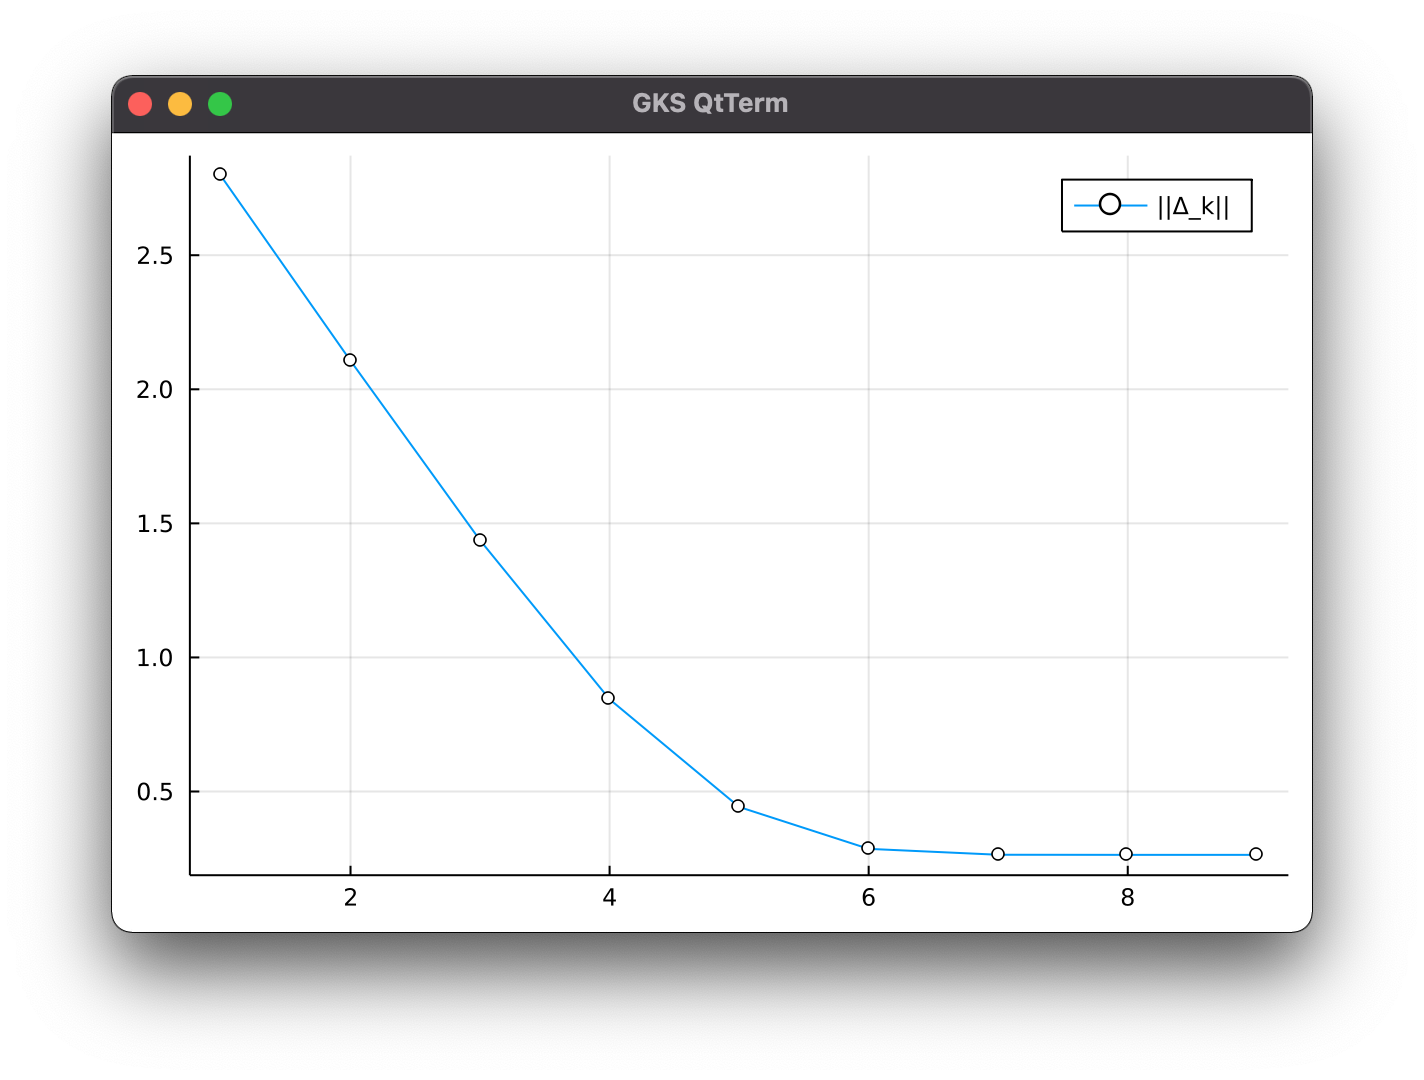
\includegraphics[scale=.5]{plot1}
    \vspace{1em}
    \begin{Verbatim}[frame=single, label=Julia REPL for finding Alpha, numbers=left, fontsize=\small, xleftmargin=0cm, framesep=3mm]
        julia> include("polar.jl")
        Slope between last two points: Alpha = -1.0004229223103496
    \end{Verbatim}
    \vspace{1em}
    \bigbreak\dotfill\bigbreak
    \section*{1d}
    Let $W$ be the limit of $X_k$ as $k \to \infty$. Numerically check whether $W$ is an orthogonal matrix by computing $X_T^\top X_k$ for $k = 8, 9, 10$. What are your conclusions?
    \vspace{1em}
    \begin{Verbatim}[frame=single, label=Check orthogonality of W, numbers=left, fontsize=\small, xleftmargin=0cm, framesep=3mm]
        #######################################
        # 1d.
  
        # calculate X_k for k = 8, 9, 10
        X_8_9_10 = [pol_driver(copy(A), k) for k = 8:10]
  
        # helper method to calculate X^T * X
        check_orth = (X) -> X' * X;
  
        # display the resulting matrices
        map(x -> display(check_orth(x)), X_8_9_10)
    \end{Verbatim}
    \vspace{1em}
    \begin{Verbatim}[frame=single, label=Julia REPL for resulting matrices, numbers=left, fontsize=\small, xleftmargin=0cm, framesep=3mm]
        julia> include("polar.jl")
        4×4 Matrix{Float64}:
          1.0          -2.57131e-14  -1.41068e-15   2.46364e-15
         -2.57131e-14   1.0           3.54173e-15  -6.04376e-15
         -1.41068e-15   3.54173e-15   1.0          -3.81e-16
          2.46364e-15  -6.04376e-15  -3.81e-16      1.0
        4×4 Matrix{Float64}:
         1.0           1.34121e-16   3.76323e-17   9.75894e-18
         1.34121e-16   1.0          -3.37948e-17  -4.60842e-17
         3.76323e-17  -3.37948e-17   1.0           2.65522e-17
         9.75894e-18  -4.60842e-17   2.65522e-17   1.0
        4×4 Matrix{Float64}:
          1.0           2.34459e-17  -4.79178e-17  -1.14298e-17
          2.34459e-17   1.0          -3.4489e-17    3.71826e-17
         -4.79178e-17  -3.4489e-17    1.0           7.58685e-17
         -1.14298e-17   3.71826e-17   7.58685e-17   1.0
    \end{Verbatim}
    Because the resulting matrices after multiplying $X_8, X_9,$ and $X_{10}$ by their transpose are very, very close to the identity matrix, clearly each matrix is orthogonal.

    \newpage

    \section*{1e}
    Define $P = W^{-1}A$ so that $A = WP$. This is called the polar decomposition of $A$. Use the built-in Julia function \texttt{eigvals} to find the eigenvlues of $P$ and $A$. Are the eigenvalues of $A$ positive? What about the eigenvalues of $P$?
    \vspace{1em}
    \begin{Verbatim}[frame=single, label=Find and display eigenvalues of P and A, numbers=left, fontsize=\small, xleftmargin=0cm, framesep=3mm]
        #######################################
        # 1e.
  
        W = X_8_9_10[3]
        P = inv(W) * copy(A)
        println("Eigenvalues of P = $(eigvals(P))");
        println("Eigenvalues of A = $(eigvals(copy(A)))");
    \end{Verbatim}
    \vspace{1em}
    \begin{Verbatim}[frame=single, label=Julia REPL for eigenvalues of P and A, numbers=left, fontsize=\small, xleftmargin=-.0cm, xrightmargin=-.0cm, framesep=3mm]
    Eigenvalues of P = [0.03086137273259231, 0.19890329211534932,
                        0.664894706530955, 0.964105847552981]

    Eigenvalues of A = ComplexF64[-0.20699017509306217 - 0.2067450022872031im,
                                  -0.20699017509306217 + 0.2067450022872031im,
                                  -0.05873738107811822 + 0.0im,
                                   0.7827177312642422 + 0.0im]
    \end{Verbatim}
    For the matrix $P$, we have all positive eigenvalues. But for $A$ we have $3$ negative eigenvalues and $1$ positive one. 


\end{document}
